\section{The PMBM filter}
\label{sec:pmbm}
\begin{itemize}
    \item Rule for this chapter: the standard PMBM as the literature defines it (\cite{garcia_2018_pmbm}). The choices and deviations of this work go in Chapter~\ref{sec:implementation}.
    \item Add a notation table that matches Section~\ref{sec:formulation}.
    \item The flow figure is taken from \cite{chalmers_mot_course}: redraw it, or make sure the caption and permission are in order.
\end{itemize}

Introduced by \textcite{williams_pmbm_2015}, the PMBM filter is the exact conjugate prior for the standard model assumptions in recursive multi target tracking. \textcite{garcia_2018_pmbm} and \textcite{garcia_2017_pmbm} finds that, with standard reduction techniques, the PMBM filter can be implemented and yields better performance than comparable RFS-filters on challenging tracking scenarios. 
\medskip

The following section will be an overview of the PMBM filter. We will start by defining the density that is carried, and how it is composed. We will then go over how the different components is predicted and updated given some data association. Lastly, we will go over the common reduction techniques used to keep the implementation feasible. This overview will skip the derivations, but present the resulting equations. The equations will first be stated generally, then for linear Gaussian assumptions. For further details, the reader is referred to \cite{garcia_2018_pmbm} or \cite{chalmers_mot_course}.
\medskip

\autoref{fig:pmbm_flow} shows how the densities are propagated through one recursion of the PMBM filter. We will refer back to this figure throughout as the concepts are explained further.

\begin{figure}[htbp]
    \centering
    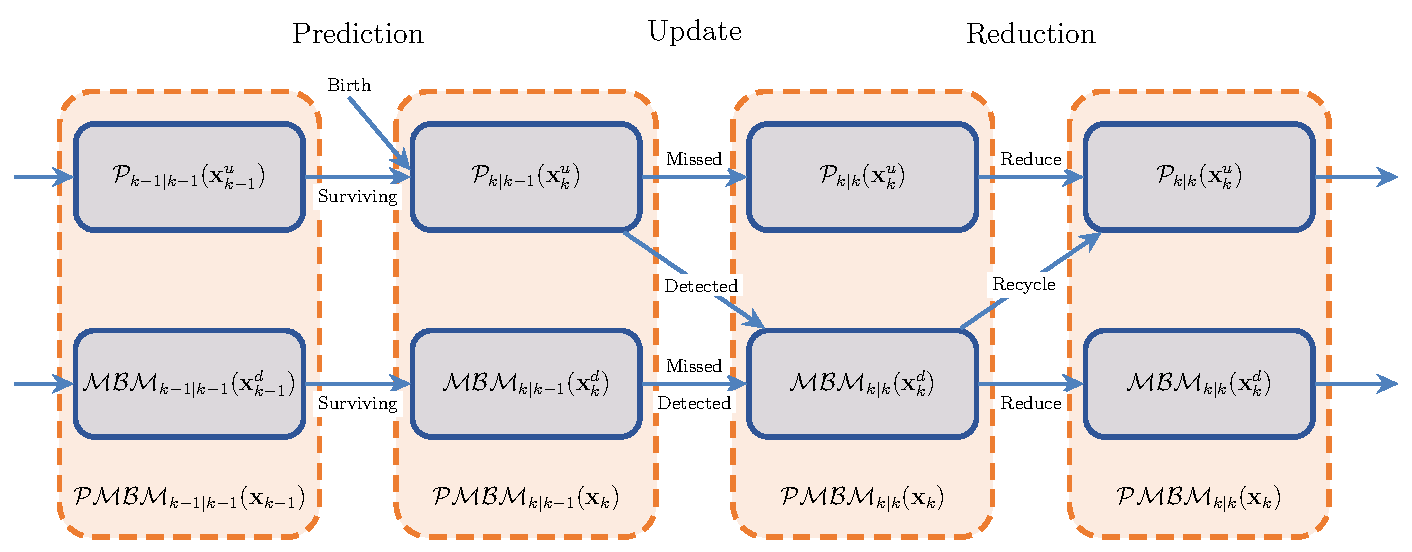
\includegraphics[width=\textwidth]{Images/pmbm_flow.pdf}
    \caption{One recursion of the PMBM filter: prediction, update and reduction. Figure taken from \cite{chalmers_mot_course}.}
    \label{fig:pmbm_flow}
\end{figure}

\subsection{PMBM density}
The PMBM density is a union of two independent random finite sets: one Poisson point process (PPP) and one Multi Bernoulli Mixture (MBM). The PPP is used for modelling new targets, the dynamics of targets not yet observed and targets forgotten by the MBM. We will come back to the last point when discussing the reduction step. The multi-Bernoulli (\textbf{MB}M) models targets we have observed at least once, their probability of existence and their state, given they exist. The mixture (MB\textbf{M}) handles uncertainty in measurement origin by considering multiple global hypotheses. \autoref{eq:pmbm} shows the factorization into the independent PPP and MBM densities. The sum goes over the disjoint union of undetected ($\mathbf{x}^u_k$) and detected ($\mathbf{x}^d_k$) target sets. That is, we sum over each possible combination of assignments of targets ($\mathbf{x}_k$), into undetected or detected targets.

\begin{equation}
  \mathcal{PMBM}_{k|k}(\mathbf{x}_k) = \sum_{\mathbf{x}^u_k \uplus \mathbf{x}^d_k = \mathbf{x}_k} \mathcal{P}_{k|k}(\mathbf{x}^u_k)\, \mathcal{MBM}_{k|k}(\mathbf{x}^d_k),
  \label{eq:pmbm}
\end{equation}
\medskip

\subsubsection{Birth and undetected Poisson point process}
\autoref{eq:ppp} shows the pdf of the PPP. $\lambda^u_{k|k}(x)$ is the Poisson intensity, which tells us where we expect new or undetected targets. It is normal to parameterize the Poisson intensity by Gaussian mixtures. One for the undetected targets, as shown in \autoref{eq:ppp_gm}, and one for the birth process, similar, but not repeated.

\begin{equation}
  \mathcal{P}_{k|k}(\mathbf{x}^u_k) = e^{-\int \lambda^u_{k|k}(x)\,\mathrm{d}x} \prod_{x \in \mathbf{x}^u_k} \lambda^u_{k|k}(x),
  \label{eq:ppp}
\end{equation}

\begin{equation}
  \lambda^u_{k|k}(x) = \sum_{h=1}^{H_{k|k}} w^{u,h}_{k|k}\, \mathcal{N}\big(x;\, \mu^{u,h}_{k|k},\, P^{u,h}_{k|k}\big),
  \label{eq:ppp_gm}
\end{equation}

The expected number of targets can be found by integrating the intensity over the state space. In the Gaussian case this integral is simply the sum of weights.

\begin{equation*}
    \int \lambda^u_{k|k}(x)\,\mathrm{d}x = \sum_{h} w^{u,h}_{k|k}
\end{equation*}

This means that the Gaussian mixture does not have to be a pdf, where the weights sum to one. Another common parameterization of the birth process, is to make it uniform inside the FOV. The Gaussian-mixture recursion is then no longer exact, since the product of a uniform intensity and a Gaussian likelihood is a truncated Gaussian. However, when the surveillance region is large compared to the measurement noise the truncation is negligible and the result is well approximated by a Gaussian.
\medskip

\subsubsection{The Multi Bernoulli Mixture}
The MBM holds different hypotheses of states for the detected targets. Multiple hypotheses are needed because of ambiguity of measurement to target association. Also, a target being detected does not mean that it is guaranteed to actually exist, which is handled by the existence probabilities. The MBM pdf is shown in \autoref{eq:mbm}, where $\mathcal{A}_{k|k}$ is the set of global hypotheses and $w^{a}_{k|k}$ is the weight of said hypotheses. Each global hypothesis weight is proportional to a product of local hypotheses weights and the weight of global hypotheses must sum to one (\autoref{eq:weights}). Just as in \autoref{eq:pmbm}, each global hypothesis is a union of independent Bernoulli random finite sets. This yields the same ``sum of combinations'' formula, but with $n$ sets instead of two.

\begin{equation}
  \mathcal{MBM}_{k|k}(\mathbf{x}^d_k) = \sum_{a \in \mathcal{A}_{k|k}} w^{a}_{k|k} \sum_{\mathbf{x}^1 \uplus \cdots \uplus \mathbf{x}^{n} = \mathbf{x}^d_k} \prod_{i=1}^{n} \mathcal{B}^{i,a^i}_{k|k}(\mathbf{x}^i), 
  \label{eq:mbm}
\end{equation}

\begin{equation}
  w^{a}_{k|k} \propto \prod_{i=1}^{n} w^{i,a^i}_{k|k},
  \qquad
  \sum_{a \in \mathcal{A}_{k|k}} w^{a}_{k|k} = 1.
  \label{eq:weights}
\end{equation}

The Bernoulli densities are shown in \autoref{eq:bernoulli}. Within each local hypothesis $a^i$, the target either exists or does not exist. This is handled by that specific targets existence probability within the local hypothesis ($r^{i,a^i}_{k|k}$). Given a target exists, it is distributed according to $p^{i,a^i}_{k|k}(x)$, within the specific local hypothesis.

\begin{equation}
  \mathcal{B}^{i,a^i}_{k|k}(\mathbf{x}) =
  \begin{cases}
    1 - r^{i,a^i}_{k|k}, & \mathbf{x} = \emptyset, \\
    r^{i,a^i}_{k|k}\, p^{i,a^i}_{k|k}(x), & \mathbf{x} = \{x\}, \\
    0, & \text{otherwise},
  \end{cases}
  \label{eq:bernoulli}
\end{equation}

It is common for the state density $p^{i,a^i}_{k|k}(x)$ to be assumed Gaussian.


\subsection{PMBM prediction}
The PMBM prediction follow from the model assumptions outlined in the problem formulation (\autoref{sec:formulation}). The most important result is that components can be predicted independently. This is because the model assumes that targets survive, move and appear independently of each other. The two parts of the model for prediction are the probability of survival and motion model. In the general case $p_S(x_{k-1})$ can be state dependent and $f(x_k \mid x_{k-1})$ non-linear.
\medskip

\subsubsection{PPP prediction}
As seen in \autoref{eq:pred_ppp}, PPP prediction consists of predicting the undetected targets and adding the birth density. Since targets are not guaranteed to survive until new measurements arrive, $p_S$ enter the Chapman-Kolmogorov integral.

\begin{equation}
  \lambda^u_{k|k-1}(x_k) = \lambda^b_k(x_k)
    + \int f(x_k \mid x_{k-1})\, p_S(x_{k-1})\, \lambda^u_{k-1|k-1}(x_{k-1})\,\mathrm{d}x_{k-1}.
  \label{eq:pred_ppp}
\end{equation}

Applying the linear Gaussian motion model and assuming constant $P_S$ gives the predicted density shown in \autoref{eq:lg_ppp_pred}. Each of the ${H_{k-1|k-1}}$ undetected components is predicted by the standard Kalman filter prediction and their weights are multiplied by the probability of survival. 

\begin{equation}
\begin{split}
  \lambda^u_{k|k-1}(x) = \lambda^b_k(x)
    &+ \sum_{h=1}^{H_{k-1|k-1}} p_S\, w^{u,h}_{k-1|k-1} \\
    &\times \mathcal{N}\big(x;\, F \mu^{u,h}_{k-1|k-1},\,
      F P^{u,h}_{k-1|k-1} F^{\mathsf{T}} + Q\big),
\end{split}
\label{eq:lg_ppp_pred}
\end{equation}

\subsubsection{MBM prediction}
MBM prediction follow the same model assumptions as the PPP. This means each Bernoulli can be predicted independently, shown in \autoref{eq:pred_w} through \ref{eq:pred_p}. Notice the normalization constant in \autoref{eq:pred_p} being the same integral as in \autoref{eq:pred_r}. The weights are unchanged through the prediction. This makes sense since only new measurements can give information about which previous associations are more likely. 

\begin{align}
  w^{i,a^i}_{k|k-1} &= w^{i,a^i}_{k-1|k-1}, \label{eq:pred_w} \\
  r^{i,a^i}_{k|k-1} &= r^{i,a^i}_{k-1|k-1}
    \int p_S(x_{k-1})\, p^{i,a^i}_{k-1|k-1}(x_{k-1})\,\mathrm{d}x_{k-1}, \label{eq:pred_r} \\
  p^{i,a^i}_{k|k-1}(x_k) &=
    \frac{\int f(x_k \mid x_{k-1})\, p_S(x_{k-1})\, p^{i,a^i}_{k-1|k-1}(x_{k-1})\,\mathrm{d}x_{k-1}}
         {\int p_S(x_{k-1})\, p^{i,a^i}_{k-1|k-1}(x_{k-1})\,\mathrm{d}x_{k-1}}. \label{eq:pred_p}
\end{align}

When applying linear Gaussian and constant $P_S$ assumptions, the integral simplify to standard Kalman filter predictions for each Bernoulli component. The existence probability gets multiplied by the probability of survival and the weights remain unchanged.

\begin{align*}
  w^{i,a^i}_{k|k-1} &= w^{i,a^i}_{k-1|k-1}, \\
  r^{i,a^i}_{k|k-1} &= p_S\, r^{i,a^i}_{k-1|k-1}, \\
  p^{i,a^i}_{k|k-1}(x) &= \mathcal{N}\big(x;\, F \mu^{i,a^i}_{k-1|k-1},\,
    F P^{i,a^i}_{k-1|k-1} F^{\mathsf{T}} + Q\big).
\end{align*}

\subsection{PMBM update}
\label{sec:pmbm-update}
\begin{itemize}
    \item Fix the notation: \autoref{eq:upd_mbm_d_w} and \autoref{eq:upd_mbm_d_p} mix $g(z \mid x)$ and $h(z \mid x)$; use $h$ as in Section~\ref{sec:formulation}. Use $\PD$ and $\PS$ consistently instead of $p_D$ and $p_S$.
    \item State at the start that this section gives the \emph{single-target} (local) hypotheses; how they combine into global hypotheses follows in Section~\ref{sec:pmbm-da}.
\end{itemize}

Having used birth, survival and a motion model to predict in the absence of measurement, we will now move on to inference from measurements. \autoref{fig:pmbm_flow} introduces the vocabulary for the section: detections and missed detections. This is also the way hypotheses evolve, as each measurement can come from an existing target, a new target or clutter. 
\medskip

To limit the number of new hypotheses generated, gating must be performed to discard very unlikely measurement $\leftrightarrow$ target combinations. This is a prerequisite to the update, so only gated measurements will be used in each specific update.
\medskip

\subsubsection{PPP update: Missed detection}
The probability of detection ($p_D$), splits the PPP into undetected and detected hypotheses. To reflect the missed detection hypotheses, each component of the intensity is scaled by the probability of missed detection (\autoref{eq:upd_ppp_md}). This is done for each component, regardless of whether it gated any measurements. The logic behind this is that the hypotheses covering detected targets are handled by the new Bernoullis described next.

\begin{equation}
  \lambda^u_{k|k}(x) = \big(1 - p_D(x)\big)\, \lambda^u_{k|k-1}(x).
  \label{eq:upd_ppp_md}
\end{equation}

Assuming constant $p_D$, only the weights of the Gaussian mixture change. The means and covariances remain unchanged. 

\begin{equation*}
  w^{u,h}_{k|k} = (1 - p_D)\, w^{u,h}_{k|k-1}, \qquad
  \mu^{u,h}_{k|k} = \mu^{u,h}_{k|k-1}, \qquad
  P^{u,h}_{k|k} = P^{u,h}_{k|k-1}.
\end{equation*}
\medskip

\subsubsection{PPP update: Detected (new target)}
Every measurement $z^j_k$ may be from a new target and thanks to the undetected PPP, we already have a prior for this target. For each measurement we create a Bernoulli with two local hypotheses. In $a^i = 1$, $z^j_k$ is associated to a previously detected target, and the new target therefore does not exist. Since a global hypothesis consists of picking a local hypothesis for each Bernoulli, this option must also be included (\autoref{eq:upd_ppp_d_none}). The second hypothesis, $a^i = 2$, covers the scenario where $z^j_k$ originates from either clutter or a new target. The uncertainty of origin is captured in the existence probability, as can be seen in \autoref{eq:upd_ppp_d_r}.

\begin{align}
  w^{i,1}_{k|k} &= 1, \qquad r^{i,1}_{k|k} = 0, \label{eq:upd_ppp_d_none}\\
  w^{i,2}_{k|k} &= e^j_k + \lambda^c(z^j_k), \label{eq:upd_ppp_d_w}\\
  r^{i,2}_{k|k} &= \frac{e^j_k}{e^j_k + \lambda^c(z^j_k)}, \label{eq:upd_ppp_d_r}\\
  p^{i,2}_{k|k}(x) &= \frac{p_D(x)\, h(z^j_k \mid x)\, \lambda^u_{k|k-1}(x)}{e^j_k}, \label{eq:upd_ppp_d_p}
\end{align}
where $e^j_k$ is the likelihood of $z^j_k$ given that it is the first detection of a previously undetected target.
\begin{equation}
  e^j_k = \int p_D(x)\, h(z^j_k \mid x)\, \lambda^u_{k|k-1}(x)\,\mathrm{d}x .
  \label{eq:upd_ppp_d_e}
\end{equation}

Using constant $p_D$, linear Gaussian assumptions, and the measurement model $h(z \mid x) = \mathcal{N}(z;\, Hx,\, R)$, each PPP mixture component that gates measurement $z^j_k$ is updated with the standard Kalman filter update. 

\begin{align*}
  \hat z^{u,h}_{k|k-1} &= H \mu^{u,h}_{k|k-1}, \\
  S^{u,h}_k &= H P^{u,h}_{k|k-1} H^{\mathsf{T}} + R, \\
  K^{u,h}_k &= P^{u,h}_{k|k-1} H^{\mathsf{T}} \big(S^{u,h}_k\big)^{-1}, \\
  \tilde\mu^{h,j}_k &= \mu^{u,h}_{k|k-1} + K^{u,h}_k \big(z^j_k - \hat z^{u,h}_{k|k-1}\big), \\
  \tilde P^{h}_k &= \big(I - K^{u,h}_k H\big) P^{u,h}_{k|k-1}.
\end{align*}

The likelihood in \autoref{eq:upd_ppp_d_e} now becomes a weighted sum over the gated components. The weight and existence probability are the same as in \autoref{eq:upd_ppp_d_w} and \autoref{eq:upd_ppp_d_r}, but using this measurement likelihood instead.

\begin{equation*}
  e^j_k = p_D \sum_{h \in \mathcal{H}^j} w^{u,h}_{k|k-1}\,
    \mathcal{N}\big(z^j_k;\, \hat z^{u,h}_{k|k-1},\, S^{u,h}_k\big).
\end{equation*}

The posterior density in \autoref{eq:upd_ppp_d_p} is now a Gaussian mixture with weights $\beta^{h,j}_k$. Each mixture component comes from a PPP component which gated the measurement. For complexity reasons, we would like to have a single Gaussian represent the new target. Moment matching is therefore performed to reduce the mixture to a single Gaussian.

\begin{align*}
  \beta^{h,j}_k &= \frac{p_D\, w^{u,h}_{k|k-1}\,
    \mathcal{N}\big(z^j_k;\, \hat z^{u,h}_{k|k-1},\, S^{u,h}_k\big)}{e^j_k}, \\
  \mu^{i,2}_{k|k} &= \sum_{h \in \mathcal{H}^j} \beta^{h,j}_k\, \tilde\mu^{h,j}_k, \\
  P^{i,2}_{k|k} &= \sum_{h \in \mathcal{H}^j} \beta^{h,j}_k
    \Big[\tilde P^{h}_k + \big(\tilde\mu^{h,j}_k - \mu^{i,2}_{k|k}\big)
    \big(\tilde\mu^{h,j}_k - \mu^{i,2}_{k|k}\big)^{\mathsf{T}}\Big].
\end{align*}
\medskip

\subsubsection{MBM update: Missed detection}
All local hypotheses $a^i$ need to create a missed detection hypothesis, denoted $(a^i, 0)$. The reason is that all measurements can be generated by either new or other existing targets no matter how many measurements a hypothesis gates. \autoref{eq:upd_mbm_md_w} to \ref{eq:upd_mbm_md_p} show the updated parameters. Notice that in the absence of measurements, only information can be gained from $p_D(x)$. 

\begin{align}
  w^{i,(a^i,0)}_{k|k} &= w^{i,a^i}_{k|k-1}
    \Big(1 - r^{i,a^i}_{k|k-1} + r^{i,a^i}_{k|k-1}
    \int \big(1 - p_D(x)\big)\, p^{i,a^i}_{k|k-1}(x)\,\mathrm{d}x\Big), \label{eq:upd_mbm_md_w}\\
  r^{i,(a^i,0)}_{k|k} &= \frac{r^{i,a^i}_{k|k-1} \int \big(1 - p_D(x)\big)\, p^{i,a^i}_{k|k-1}(x)\,\mathrm{d}x}
    {1 - r^{i,a^i}_{k|k-1} + r^{i,a^i}_{k|k-1} \int \big(1 - p_D(x)\big)\, p^{i,a^i}_{k|k-1}(x)\,\mathrm{d}x}, \label{eq:upd_mbm_md_r}\\
  p^{i,(a^i,0)}_{k|k}(x) &= \frac{\big(1 - p_D(x)\big)\, p^{i,a^i}_{k|k-1}(x)}
    {\int \big(1 - p_D(x')\big)\, p^{i,a^i}_{k|k-1}(x')\,\mathrm{d}x'}. \label{eq:upd_mbm_md_p}
\end{align}

With constant $p_D$ no information can update the state density and the state density is unchanged. However, the absence of measurement results in a reduction in both weight and existence probability.

\begin{align*}
  w^{i,(a^i,0)}_{k|k} &= w^{i,a^i}_{k|k-1} \big(1 - r^{i,a^i}_{k|k-1}\, p_D\big), \\
  r^{i,(a^i,0)}_{k|k} &= \frac{r^{i,a^i}_{k|k-1}\,(1 - p_D)}{1 - r^{i,a^i}_{k|k-1}\, p_D}, \\
  \mu^{i,(a^i,0)}_{k|k} &= \mu^{i,a^i}_{k|k-1}, \qquad
  P^{i,(a^i,0)}_{k|k} = P^{i,a^i}_{k|k-1}.
\end{align*}
\medskip

\subsubsection{MBM update: Detected}
For each measurement $z^j_k$ inside the gate of local hypothesis $a^i$, a detection hypothesis $(a^i, j)$ is created. This is because you cannot know which measurement belong to the target. Given that the target generated a measurement, it exists with certainty. It therefore gets an existence probability of one within this local hypothesis.

\begin{align}
  w^{i,(a^i,j)}_{k|k} &= w^{i,a^i}_{k|k-1}\, r^{i,a^i}_{k|k-1}
    \int p_D(x)\, g(z^j_k \mid x)\, p^{i,a^i}_{k|k-1}(x)\,\mathrm{d}x, \label{eq:upd_mbm_d_w}\\
  r^{i,(a^i,j)}_{k|k} &= 1, \label{eq:upd_mbm_d_r}\\
  p^{i,(a^i,j)}_{k|k}(x) &= \frac{p_D(x)\, h(z^j_k \mid x)\, p^{i,a^i}_{k|k-1}(x)}
    {\int p_D(x')\, g(z^j_k \mid x')\, p^{i,a^i}_{k|k-1}(x')\,\mathrm{d}x'}. \label{eq:upd_mbm_d_p}
\end{align}

Under linear Gaussian assumptions and constant $p_D$, this is a standard Kalman filter update, where the weight is scaled by the predicted measurement likelihood.

\begin{align*}
  \hat z^{i,a^i}_{k|k-1} &= H \mu^{i,a^i}_{k|k-1}, \\
  S^{i,a^i}_k &= H P^{i,a^i}_{k|k-1} H^{\mathsf{T}} + R, \\
  K^{i,a^i}_k &= P^{i,a^i}_{k|k-1} H^{\mathsf{T}} \big(S^{i,a^i}_k\big)^{-1}, \\
  w^{i,(a^i,j)}_{k|k} &= w^{i,a^i}_{k|k-1}\, r^{i,a^i}_{k|k-1}\, p_D\,
    \mathcal{N}\big(z^j_k;\, \hat z^{i,a^i}_{k|k-1},\, S^{i,a^i}_k\big), \\
  r^{i,(a^i,j)}_{k|k} &= 1, \\
  \mu^{i,(a^i,j)}_{k|k} &= \mu^{i,a^i}_{k|k-1} + K^{i,a^i}_k \big(z^j_k - \hat z^{i,a^i}_{k|k-1}\big), \\
  P^{i,(a^i,j)}_{k|k} &= \big(I - K^{i,a^i}_k H\big) P^{i,a^i}_{k|k-1}.
\end{align*}


% =====================================================================
\subsection{Track-oriented representation}
\label{sec:pmbm-representation}
\label{sec:anatomy-hyp}
\begin{itemize}
    \item Builds on the HO/TO discussion in Section~\ref{sec:families}; the PMBM stores its hypotheses track-oriented.
    \item Each track is a tree of single-target hypotheses, one level per scan; the leaves are its current local hypotheses.
    \item A global hypothesis is a look-up table: one leaf per track, or none.
    \item Why it scales: a leaf is stored once and shared by many global hypotheses; pruning a global hypothesis removes the leaves nobody references any more.
    \item The hybrid: track-oriented storage, hypothesis-oriented generation (Murty per prior global hypothesis, Section~\ref{sec:pmbm-da}), as in \cite{garcia_2018_pmbm} and in this work.
    \item New figure: one small PMBM example drawn as hypothesis trees, with the table of global hypotheses as look-ups into the leaves. The HO/TO comparison figure is in Section~\ref{sec:families}.
\end{itemize}

% =====================================================================
\subsection{Global hypotheses and data association}
\label{sec:pmbm-da}
\begin{itemize}
    \item The local hypotheses of Section~\ref{sec:pmbm-update} combine into global hypotheses: each prior global hypothesis picks one child per track, and each measurement is used exactly once, either by an existing track or by its own new Bernoulli (new target or clutter).
    \item The weight of a new global hypothesis is the product of the chosen local weights, normalized over all global hypotheses.
    \item The number of new global hypotheses grows combinatorially, so only the $k$ best are generated.
    \item The assignment formulation (\cite{garcia_2018_pmbm}): a cost matrix with one row per measurement, a block of existing tracks and a diagonal block of new Bernoullis, with $-\infty$ (infeasible) outside the gates and off the diagonal. Costs are normalized by the missed-detection weights, so ``no measurement'' is implicit.
    \item $k$-best assignments with Murty's method \cite{Murty}, run once per prior global hypothesis, with a budget proportional to the prior's weight.
    \item Cost: about $k \cdot n^3$ per prior hypothesis, so large clusters are expensive (link to Section~\ref{sec:complexity}). Alternative: Gibbs sampling \cite{gibbs_glmb}.
\end{itemize}



% =====================================================================
\subsection{PMBM reduction}
\label{sec:pmbm-reduction}
\begin{itemize}
    \item Gating (introduced in Section~\ref{sec:anatomy}): Mahalanobis gate, gate probability $P_G$, and what is lost by ignoring it.
    \item Pruning: remove global hypotheses whose weight is below a threshold.
    \item Capping: keep at most $N_h$ global hypotheses.
    \item Bernoulli pruning: remove Bernoullis with existence probability below a threshold.
    \item N-scan pruning versus limiting the tree depth (the latter forgets history without forcing a decision).
    \item Recycling \cite{williams_pmbm_2015}: Bernoullis with low existence are approximated as Poisson components. Mass is moved, not lost, and the number of Bernoullis and hypotheses falls.
    \item Poisson intensity: prune small components; merge similar components (mixture reduction).
    \item Moment matching of new Bernoullis (already in Section~\ref{sec:pmbm-update}) is also a reduction; refer back to it.
\end{itemize}

% =====================================================================
\subsection{Clustering}
\label{sec:pmbm-clustering}
\begin{itemize}
    \item Given the gates, tracks that share no measurement are independent: the MBM factorizes into a product of per-cluster MBMs, each with its own list of global hypotheses. The Poisson intensity is shared.
    \item Exact given the gating; only the truncation of each list is an approximation.
    \item Benefit: one short hypothesis list per cluster instead of one list over the product of all clusters; capping applies per cluster.
    \item Merge: clusters that gate a common measurement form one group, whose hypothesis list is the product of the clusters' lists.
    \item Split: when tracks no longer share a measurement in their histories, they become independent again (Kurien's rule).
    \item Breaking clusters up again is what keeps them small; it works best in sparse scenes (moved here from Section~\ref{sec:complexity}).
    \item The concrete merge and split rules of this work, and their approximations, are in Chapter~\ref{sec:implementation}.
\end{itemize}

% =====================================================================
\subsection{Estimation}
\label{sec:pmbm-estimation}
\begin{itemize}
    \item The usual estimator: take the best global hypothesis and report the Bernoullis with existence probability above a threshold (\cite{garcia_2018_pmbm}).
    \item Alternatives: estimators based on the MAP cardinality, or on existence-weighted (marginal) probabilities.
    \item Track identity is the root of the tree. A trajectory is stitched from per-scan estimates, so a switch of the best hypothesis can create track switches.
    \item Trajectory PMBM as an alternative: one sentence, further work.
\end{itemize}
